\documentclass{beamer}
\usepackage[utf8]{inputenc} 
\title{Rozpoznawanie obrazów}
\author{Paweł Kumorowski}
\date{\today}
\usepackage{amsfonts}
\usepackage[MeX]{polski}
\usepackage{graphicx}
\begin{document}
\frame{\titlepage}


\begin{frame}
\frametitle{Spis Treści}
\tableofcontents
\end{frame}


\section{Wstęp}
\begin{frame}{Rozpoznawanie obrazów}

\begin{figure}
	\centering
		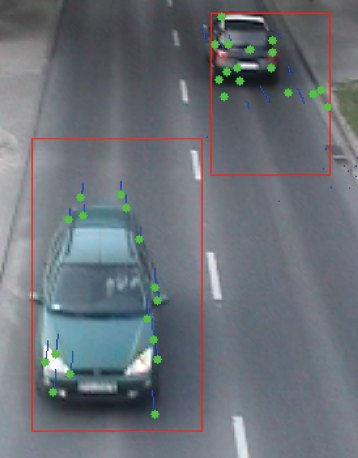
\includegraphics[width=0.3\textwidth]{samochod.jpg}
		\caption{System rozpoznający obiekty}
\end{figure}

\begin{itemize}
\item Rozpoznawanie obrazu --- przetwarzanie obrazu przez maszynę za pomocą urządzeń zewnętrznych (np. skaner) w opis cyfrowy tegoż obrazu w celu dalszego przetwarzania.
\end{itemize}
\end{frame}


\section{Wymagania}
\begin{frame}{Wymagania}
\begin{itemize}
\item Do poprawnego rozpoznania tego co znajduje się na obrazie wymagana jest wstępna ,,wiedza''. Człowiek wiedzę potrzebną mu do poprawnego rozpoznawania i~rozumienia istoty rzeczy zbiera bezwiednie poprzez całe swoje życie, maszynę zaś trzeba tej wiedzy "nauczyć".
\pause
\item Sam proces uczenia maszyny może polegać na utworzeniu odpowiedniej bazy danych zawierającej niezbędne reguły i~opis cech przedmiotu.
\end{itemize}
\end{frame}

\section{Prawdziwy cel}
\begin{frame}{Prawdziwy cel}
\begin{itemize}
\item W rozpoznawaniu obrazów bazującym na statystyce naszym celem jest oszacowanie prawdopodobieństwa, czy obiekt, któremu ,,się przyglądamy'' jest tym czy innym obiektem którego opis znajduje się wśród wiedzy posiadanej przez nasz system. 
\pause
\item W związku z tym dążymy do osiągnięcia 100\% pewności co do zaklasyfikowania obiektu, jednakże tej 100\% pewności nigdy nie osiągamy.
\end{itemize}
\end{frame}

\section{Błąd klasyfikacji}
\begin{frame}{Błąd klasyfikacji}
\begin{itemize}
\item Zadaniem twórcy systemu rozpoznawania obrazu jest skonstruowanie takiego algorytmu, który będzie minimalizował błąd klasyfikacji obiektu prezentowanego na obrazie, bądź całego obrazu.
\pause
\item Zadanie to nie należy do trywialnych, dlatego zakłada się minimalizacje błędu klasyfikacji, a nie całkowite jego wyeliminowanie.
\end{itemize}
\end{frame}

\section{Ograniczenia narzucane systemowi}
\begin{frame}{Ograniczenia narzucane systemowi}\
Często, aby usprawnić oraz uprościć działanie systemu rozpoznawania obrazów wprowadza się pewne ograniczenia.
\pause
\begin{itemize}
\item Pytania zadawane systemowi sprawdzają się do sformowania jaki obiekt najprawdopodobniej występuje na obrazie, a odpowiedzią jest obiekt klasy która w drodze ewaluacji dostał najwyższą notę prawdopodobieństwa.
\pause
\item Zestaw danych opisujących obiekt przeznaczony do rozpoznania ograniczone są do skończonego zestawu cech.
\end{itemize}
\end{frame}



\end{document}

